\documentclass[a4paper,12pt,twoside,openright,titlepage]{book}

%Additional packages
\usepackage[utf8]{inputenc}
\usepackage[T1]{fontenc}
\usepackage[dutch,english]{babel}
\usepackage{imakeidx}
\usepackage{syntonly}
\usepackage[official]{eurosym}
%\usepackage[graphicx]
\usepackage{graphicx}
\graphicspath{ {./images/} }
\usepackage{float}
\usepackage{xurl}
\usepackage{hyperref}
\hypersetup{colorlinks=true, linkcolor=blue, citecolor=blue, filecolor=blue, urlcolor=blue, pdftitle=, pdfauthor=, pdfsubject=, pdfkeywords=}
\usepackage{tabularx}
\usepackage[table]{xcolor} % Table colors
\usepackage{scrextend}
\addtokomafont{labelinglabel}{\sffamily}
\usepackage{listings}
\usepackage{adjustbox}
\usepackage{color}
\usepackage{csquotes}
\usepackage{siunitx} % On Debian do install texlive-science

% Define colors
\definecolor{ashgrey}{rgb}{0.7, 0.75, 0.71}

% Listing style
\lstset{
  backgroundcolor=\color{ashgrey}, % choose the background color; you must add \usepackage{color} or \usepackage{xcolor}; should come as last argument
  basicstyle=\footnotesize,        % the size of the fonts that are used for the code
  breakatwhitespace=true,          % sets if automatic breaks should only happen at whitespace
  breaklines=true,                 % sets automatic line breaking
  extendedchars=true,              % lets you use non-ASCII characters; for 8-bits encodings only, does not work with UTF-8
  frame=single,	                   % adds a frame around the code
  rulecolor=\color{black},         % if not set, the frame-color may be changed on line-breaks within not-black text (e.g. comments (green here))
  keepspaces=true,                 % keeps spaces in text, useful for keeping indentation of code (possibly needs columns=flexible)
  columns=fullflexible,		   % make copy and paste possible
  showstringspaces=false,          % if true show spaces in strings adding particular underscores
  showspaces=false,                % if true show spaces everywhere adding particular underscores; it does not override 'showstringspaces'
}

% Uncomment for production
% \syntaxonly

% Style
\pagestyle{headings}

% Turn on indexing
\makeindex[intoc]

% Define document
\author{D. Leeuw}
\title{Backup}
\date{\today\\v.1.0.0}

\begin{document}
\selectlanguage{dutch}

\maketitle

\copyright\ 2024 Dennis Leeuw\\

\begin{figure}

\includegraphics[width=0.3\textwidth]{CC-BY-SA-NC.png}
\end{figure}

\bigskip

Dit werk is uitgegeven onder de Creative Commons BY-NC-SA Licentie en laat anderen toe het werk te kopi\"eren, distribueren, vertonen, op te voeren, en om afgeleid materiaal te maken, zolang de auteurs en uitgever worden vermeld als maker van het werk, het werk niet commercieel gebruikt wordt en afgeleide werken onder identieke voorwaarden worden verspreid.


%%%%%%%%%%%%%%%%%%%
%%% Introductie %%%
%%%%%%%%%%%%%%%%%%%

\frontmatter
\chapter{Over dit Document}
\section{Leerdoelen}
Dit document geeft een basis uitleg over de boolean algebra in relatie tot de elektrotechniek. De verschillende Boolean functies worden beschreven aan de hand van elektronische schema's. De lezer leert dan ook wat boolean algebra is in de context van de elektrotechniek.


\section{Voorkennis}
\begin{itemize}
\item Om de uitleg te kunnen volgen die beschreven is bij de elektronische werking van de verschillende functies dient de lezer kennis te hebben van de werking van transistoren, weerstanden, spanning en stroom
\item Het is handig als de lezer enigzins vertrouwd is met het lezen van stroomschema's
\end{itemize}


%%%%%%%%%%%%%%%%%
%%% De inhoud %%%
%%%%%%%%%%%%%%%%%
\tableofcontents

\mainmatter
\chapter{Inleiding}
Onze wereld draait inmiddels om de data die we genereren. Het zijn de documenten op ons werk, de berichten op social media, de foto's op onze telefoons. Ons hele leven hangt van digitale data aan elkaar.

Onze data staat op apparaten en daar kan van alles mee gebeuren:
\begin{description}
\item [menselijke fouten] Het per ongeluk weggegooien van data, of later denken dat het toch niet weg had gemoeten
\item [natuurlijke oorzaken] Door brand of wateroverlast kunnen opslagsystemen verloren gaan of onherstelbaar beschadigd worden
\item [ouderdom] - Een harddisk of SSD kan stuk gaan door ouderdom
\item [bitrot] - Data wordt opgeslagen op een harddisk met magnetisme dat verliest na verloop van tijd zijn magnetisme en op een gegeven moment is er geen veschil meer tussen een 1 en een 0
\item [diefstal] - Apparatuur waarop de belangrijke data hebben staan kunnen gestolen worden
\item [cryptolockers] - Malware kan onze data encrypten en alleen tegen betaling krijgen we misschien de sleutel om de data te decrypten
\end{description}

Het is steeds de vraag waartegen we ons willen beschermen, wat het mag kosten en wat de eisen zijn die we stellen aan onze data. Om een goede afweging te maken is het belangrijk dat we de verschillende mogelijkheden kennen.



\chapter{Backup van data}
De meest eenvoudig vorm van backup is de kopie. Sla een kopie van een document op onder een andere naam of in een andere directorie en je kan deze terug zetten als er wat fout gegaan is met het origineel. Het nadeel van deze oplossing is dat als het opslagmedium in het systeem stuk gaat je het origineel en de kopie kwijt bent.

Een andere oplossing is het opslaan van een kopie van de data op een andere harddisk of op een USB-stick. Mocht het origineel verloren gaan of zelfs de volledige harddisk overlijden, dan heb je altijd nog een backup op de andere disk. Het is natuurlijk wel arbeidsintensief om elke keer een kopie te maken als je het origineel hebt aangepast of als je een nieuw document hebt gemaakt. Het gebeurt natuurlijk een keer dat je dat vergeet.

We zouden ook een stukje software elk uur kunnen laten draaien om een backup te maken van al onze documenten. Zo weten we zeker dat er altijd een backup is van maximaal een uur oud. Het nadeel is dat als we terug willen naar de versie van 3 uur geleden, dat die inmiddels overschreven is door de versie van 2 uur geleden.

We willen dus een kopie hebben die afhankelijk is van het tijdstip waarop de backup gemaakt is. We zouden er bijvoorbeeld voor kunnen kiezen dat de backup-software een map maakt met de datum en tijd en waarin deze een kopie zet van onze data, dan kunnen we kiezen welke versie we terug willen zetten. Het nadeel is dat we elk uur een nieuwe map krijgen met al onze data erin. De harddisk zal dus heel snel vol lopen.

Voor dit laatste probleem zijn er verschillende oplossingen:
\begin{enumerate}
\item Is het echt nodig om elk uur een kopie te maken of is \'e\'en keer per dag genoeg
\item Limiteer het aantal te bewaren mappen. Hoe ver wil je terug kunnen in de tijd?
\item Maak alleen een kopie van die data die daadwerkelijk gewijzigd is
\item Comprimeer (zip) de data
\item Dedupliceer de data - veel gebruikers slaan dezelfde documenten op, dus als twee of meer documenten hetzelfde zijn sla er dan maar 1 op in de backup
\end{enumerate}

Al deze features zijn vaak onderdeel van de huidige backup-software oplossingen. Vele leveranciers en open source programmeurs hebben zich gestort op het schrijven van de beste backup oplossing. Het loont de moeite om de verschillende producten met elkaar te vergelijken voordat je een beslissing neemt over welke backup software je wilt gaan gebruiken.



\chapter{Het veiligstellen van data}
\section{On- of Off-site}
Met een kopie van de data op dezelfde harddisk heeft dit gevolgens als de harddisk overlijdt. Het is beter om een kopie te maken op een andere harddisk. Zolang als de data binnen dezelfde omgeving blijft heet dit een on-site backup. Kortom als de lokatie afbrand hebben we nog steeds een probleem.

Een oplossing hiervoor is overbrengen van de kopie naar een andere lokatie. Dit heet dan een off-site backup. De vraag reist nu wel hoeverweg moet de backup zijn om veilig te zijn? Om deze vraag te kunnen beantwoorden moeten we ons afvragen waartegen we ons willen beschermen. Is het voldoende om ons te beschermen tegen een brand op een lokatie of moeten we de data beschermen tegen een nucleaire aanval.


\section{On- of Off-line}
Een kopie van de data kan bijvoorbeeld met \texttt{rsync} gemaakt worden van \'e\'en systeem naar een tweede. Om dit te kunnen doen moeten beide systemen aan staan. Ook bij RAID kunnen we data repliceren (mirror) naar een tweede disk. In beide gevallen spreken we van on-line data. Het voordeel van deze manier is dat de data vrijwel meteen beschikbaar is als het originele systeem stuk gaat. Het nadeel is, omdat de data on-line is, dat bijvoorbeeld cryptoware of een andere aanvaller direct ook bij de data zou kunnen. Voor RAID is dit vooral een probleem omdat de data direct gerepliceerd wordt, dus de encrypte data wordt gerepliceerd. Een systeem dat periodiek een kopie maakt is hiervoor minder gevoelig als de plek waarnaar gekopieerd wordt niet van buitenaf benaderd kan worden.

Een andere mogelijkheid is dat data off-line wordt opgeslagen. Bij dit soort systemen denken we vaak aan tapes. De backup wordt gemaakt op tape en zodra de backup klaar is wordt de tape uit de tapestreamer verwijderd. De data is dan niet meer direct benaderbaar.



\chapter{Versioning}
Versioning is het opslaan van verschillende versies van de data. Hierbij is het mogelijk om terug te gaan naar een oudere versie. Dit kan handig zijn als er wijzigingen in een document zijn aangebracht hier later toch niet gewenst zijn. Het kan gebeuren dat een compleet hoofdstuk uit een boek verwijderd wordt waarvan we later toch deze weer willen opnemen. Dan is het handig als we deze uit een oude versie kunnen terug halen.


\section{Snapshots}
Snapshotting is een vorm van versioning en is een on-site backup. Een bestandssysteem werkt met pointers naar de data. Een snapshot maakt nieuwe pointers naar de bestaande data. De data op het bestandssysteem en de data op de snapshot verwijzen dus naar dezelfde data, beide zijn gelijk. Als een bestand gewijzigd wordt dan verandert op het bestandssysteem de pointer naar de nieuwe data, terwijl de pointer vanuit de snapshot blijft staan naar de oude data. Zie figuur \ref{fig:snapshot} voor een grafische weergave van de werking van snapshots.

\begin{figure}[h]
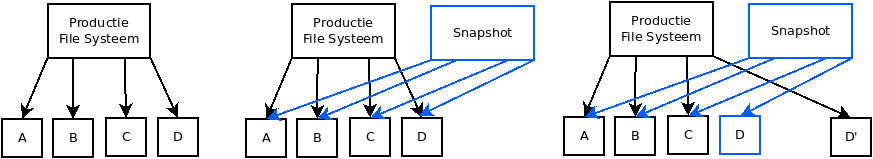
\includegraphics[width=\textwidth]{snapshot}
\centering
	\caption{Hoe snapshotting werkt}
	\label{fig:snapshot}
\end{figure}
Zo kunnen we met een minimale overhead terug naar een oude versie van onze data, welliswaar tegen de kosten van extra data gebruik op ons systeem.



\chapter{Backup schemes}
\section{Son-Father-Grandfather}
Het principe berust op het minimaliseren van het aantal backups dat wordt bewaard. De eerste backup die gemaakt wordt heet de zoon. Als er de volgende dag weer een backup gemaakt wordt dan wordt dat de zoon en de zoon heet dan vader. Wordt de dag daarop weer een backup gemaakt dan heet die nu zoon en wordt de zoon weer vader en de vader wordt grootvader. Er zijn nu drie backups van drie verschillende dagen. Bij de backup die daarna gemaakt wordt wordt de grootvader gebruikt om de backup op te schrijven. De grootvader wordt dus weer zoon, de zoon vader en de vader de nieuwe grootvader. Dit kunnen we oneindig blijven herhalen. Zodat we altijd 3 dagen terug kunnen, maar niet meer.

Een alternatief voor het zoon-vader-grootvader principe is een backup-medium voor elke dag van de week, daarmee kunnen we een week terug.


\section{Full-Differential-Incremental}
Een backup van alle data op een andere plek heet een full-backup. De meeste gebruikers werken niet elke dag aan alle documenten, maar slechts aan enkele. Als we wel elke dag alle data kopi\"eren doen we feitelijk te veel. We kunnen bezuinigen op de hoeveelheid data door alleen de gewijzigde data te kopi\"eren. We winnen zo op de ruimte die de data inneemt en ook op de tijd die het duurt om een backup te maken. Een backup van alleen de data die gewijzigd is heet een incremental-backup.

Bij een calamiteit waarbij de originele datadrager verloren gaat kost het terug zetten van de data meer tijd. Want eerst moet de full-backup terug gezet worden en daarna elke incremental die we hebben, omdat die de laatste wijzigingen bevatten.

Een tussen oplossing is het maken van een full-backup, daarna een aantal incrementals en dan een differential-backup. Een differential backup is feitelijk een samenvatting van de tussen liggende incrementals. Kortom de bestanden die gewijzigd zijn vanaf het moment dat er voor de laatste keer een full-backup is gemaakt worden weggeschreven op de differential. Dit heeft als voordeel dat bij een calamiteit de full-backup terug gezet moet worden, de differential en eventueel de daarna gekomen incrementals, maar niet meer de incrementals die tussen de full-backup en de differential zaten.

Veel bedrijven maken gebruik van deze oplossing. Op zondag wordt er een full-backup gemaakt want dan wordt er niet gewerkt en is er dus alle tijd om een volledige backup van alle data te maken. Op maandag en dinsdag worden er incrementals gemaakt en op woensdag een differential, waarna er op donderdag, vrijdag en zaterdag weer incrementals volgen.


\section{Een combinatie van de twee}
Een combinatie van full, incremental en differential backups in combinatie met het zoon-vader-grootvader principe is een veel gebruikt principe. Er zijn bijvoorbeeld 21 tapes aanwezig. 7 tapes dienen als zoon, 7 tapes als vader en 7 tapes als grootvader. De zoon tapes worden gebruikt om elke dag van de week een backup op te maken volgens een schema met full en incremental backups. De zoon tapes verplaatsen zich naar een off-site lokatie en worden daar de vader. De vader tapes worden dan grootvader en verplaatsen zich van de off-site lokatie naar de werkomgeving. De grootvader tapes worden hergebruikt als de zoon tapes. Zo is er altijd en backup. Zelfs als er tijdens transport of op de off-site lokatie wat mis gaat.



\chapter{Backup media}
Backups kunnen naar verschillende apparaten weggeschreven worden. De meest bekende oplossingen zijn harddisk (of SSD), tapes of de cloud. We zullen in dit document alleen tape en de cloud behandelen.


\section{Tape}
Een van de oudste systemen om data op te slaan is tape. Tape is niets anders dan en plastic lint dat voorzien is van magnetisch materiaal waar door een schrijfkop enen of nullen op gezet worden. Een leeskop kan die enen en nullen weer terug lezen.

Het systeem bestaat uit de tapes en een tapestreamer. De tapestreamer kan geladen worden met 1 of meer tapes. De tapestreamer schrijft of leest de tapes. Als een tape vol is kan deze vervangen worden door een lege waarop vervolg data geschreven kan worden.

Backup software kan een een kopie maken van de data en deze wegschrijven naar een tape. Als de software daarna de tapestreamer de opdracht geeft om de tape te ejecten dan is de data verder veilig tegen bijvoorbeeld overschrijven. Met een datum op de tape kunnen we altijd de data van die datum terug halen.

Tape kent een aantal voordelen:
\begin{itemize}
\item Relatief lage kosten van de tapes
\item Oneindig uitbreidbaar, we kunnen steeds nieuwe tapes kopen
\item Off-line, hacker en cryptolocker proof
\item Off-site bewaarbaar
\item Relatief lange levensduur
\item Energie zuinig, tapes hebben geen spanning nodig om hun data te behouden
\end{itemize}

Natuurlijk zijn er ook nadelen aan tapes:
\begin{itemize}
\item Ze zijn relatief traag
\item Het kan wat werk zijn om de juiste tape terug te vinden
\item Tapes maken gebruik van magnetisme om hun data op te slaan, dus zijn ze gevoelig voor bitrot
\item Omdat ze data kunnen verliezen zullen tapes eens in de zoveel tijd geconroleert moeten worden of de data nog toegankelijk is
\item Het is een relatief arbeidsintensief proces, dus zijn de arbeidsloon kosten hoog
\item Wat vaak vergeten wordt zijn de kosten voor opslag. Tapes moeten ergens opgeborgen worden.
\end{itemize}


\subsection{LTO - Linear Tape Open}
Er zijn verschillende systemen voor het maken van backups op tape. In 1990s kwamen er een open standaard ontwikkeld door Hewlett Packard Enterprise, IBM en Quantum. Deze standaard heet Linear Tape Open of afgekort LTO. Sinds dien zijn er verschillende versies op de markt gekomen. Voor een overzicht verwijzen we naar de Engelstalige Wikipedia pagina: \url{https://en.wikipedia.org/wiki/Linear_Tape-Open}.


\section{Cloud}
Veel data wordt tegenwoordig in de cloud gebackupd, denk hierbij aan alle data van de mobiele telefoons en tablets. Maar ook veel laptops kopi\"eren hun data naar de cloud van Apple of Microsoft. Het grote voordeel is dat de gebruiker zich niet druk hoeft te maken over het veilig stellen van zijn data. En als hij een nieuwe telefoon koopt (van dezelfde operating system fabrikant) dan kan hij simpel zijn data over zetten naar de nieuwe telefoon. Het nadeel is dat de data bij de fabrikant staat. Het staat op hun servers en ze zouden de data kunnen lezen, tenzij je je data encrypt hebt.



\chapter{Backup van hardware}
Ook hardware kan stuk of verloren gaan. Het is dus goed om ook hier vervanging voor te hebben. Voor harddisks (SSDs) wordt er vaak gebruik gemaakt van RAID, maar er zijn ook andere oplossingen. Deze sectie geeft hiervan enkele voorbeelden.


\section{Spare}
De meest simpele vorm van een backup voor hardware is zorgen dat er een tweede identiek exemplaar beschikbaar is binnen de organisatie. Zo kan je bijvoorbeeld snel een defecte harddisk vervangen door een nieuwe. Dit is een prima oplossing bij RAID-systemen. Vervang de defecte harddisk door een op de plank klaar liggend exemplaar en het RAID-systeem zal de disk automatisch voorzien van de data die op de defecte disk stond.


\section{Hot Standby}
Voor hele servers is het lastig als er bij een calamiteit eerst een installatie van het operating system gedaan moet worden, daarna moet de benodigde software erop gezet worden en dan moet ook nog de data op het systeem gezet worden. Sommige servers zijn zo cruciaal voor een bedrijf dat dit te lang zou duren. Dit soort servers worden meestal voorzien van een broertje met een identieke installatie en de data wordt tussen de twee servers gesynchroniseerd. Omdat beide servers aan staan heet dit een Hot Standby. Zodra de productie server omvalt kan er meteen overgeschakeld worden op de Hot Standby die dan verder functioneert als de productie server. De defecte server zal dan vervangen moeten worden voor een nieuwe Hot Standby.


\section{Virtualisatie}
Als de servers binnen een bedrijf gevirtualiseerd zijn, dan kunnen de disk images gebackupt worden. Ze kunnen bijvoorbeeld gekopieerd worden naar een andere hypervisor. Valt de eerste hypervisor uit dan kan de tweede hypervisor opgestart worden. Het kan natuurlijk ook dat als er wat met een VM gebeurd dat er dan alleen voor die ene VM overgeschakeld wordt naar de andere hypervisor.



%%%%%%%%%%%%%%%%%%%%%
%%% Index and End %%%
%%%%%%%%%%%%%%%%%%%%%
\backmatter
\printindex
\end{document}

%%% Last line %%%
